\section{Ergänzende Instrumente}

\textbf{Anhang der Kapitalgesellschaft}:
\begin{itemize}
	\item \textbf{Erläuterungs-}, \textbf{Ergänzungs-}, \textbf{Entlastungs-} (Verlagerung von Informationen in den Anhang), \textbf{Korrekturfunktion} (Angaben zur Vermeidung von Fehlinformation) für Bilanz und GuV
	\item Zwei Arten von Angaben im Anhang:
	\begin{itemize}
		\item \textbf{Pflichtangaben}:
		\begin{itemize}
			\item Angaben, die immer im Anhang zu machen sind
			\item Angaben, die aufgrund der eines Wahlrechts nicht in Bilanz oder GuV aufgenommen wurden
			\item Bilanzierungs- und Bewertungsmethoden, die auf Bilanz und GuV angewendet wurden
			\item Abweichungen von Bilanzierungs- und Bewertungsmethoden
			\item Unterschiedsbeträge
			\item Einbeziehung von Fremdkapitalzinsen in die Herstellungskosten
			\item Darstellung des Anlagevermögens mit Hilfe eines \textbf{Anlagespiegels}
			\begin{center}
				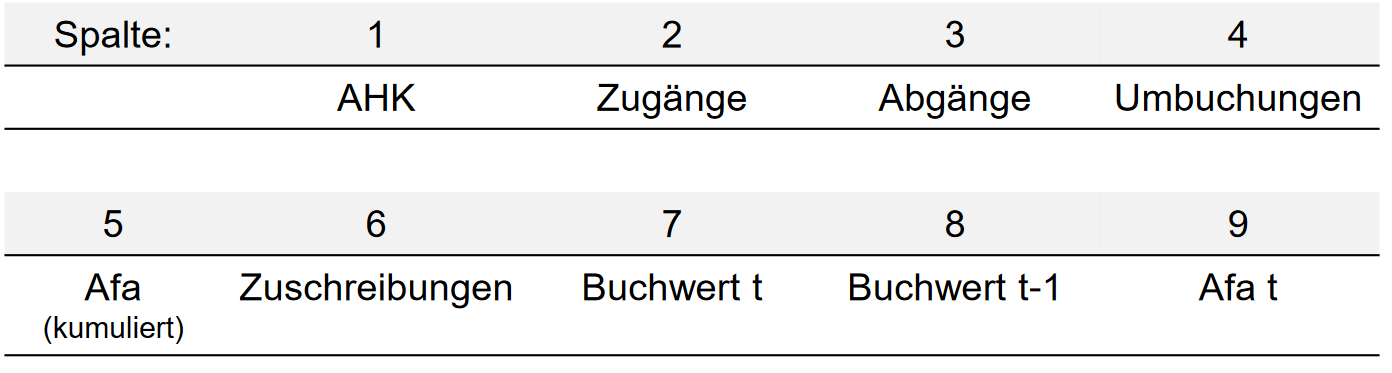
\includegraphics[width=0.7\textwidth]{images/anmirr.png}
			\end{center}
			$\rightarrow$ Darlegung von im Anlagevermögen gebundene Kapital, Altersstruktur der Vermögensgegenstände und der Entwicklung der einzelnen Posten.
		\end{itemize}
		\item \textbf{Sonstige Pflichtangaben}: 
		\begin{itemize}
			\item Fristigkeit und Besicherung der Verbindlichkeiten
			\item Informationen zu außerbilanziellen Geschäften
			\item Gesamtbeträge sonstiger finanzieller Verpflichtungen
			\item Aufgliederung der Umsatzerlöse
			\item Weitere Inhalte s. FS6/12-14
			\item
		\end{itemize}
	\end{itemize}
\end{itemize}